\documentclass{article}
\pagestyle{empty}
\usepackage{hyperref}
\usepackage{graphicx}
\usepackage{multicol}
\usepackage[margin=1in]{geometry}
\begin{document}
\begin{multicols}{2}
  \centerline{\LARGE Assignment \# 3, CSCI 480}

  \centerline{\Large Fall 2015}

\centerline{\large Due date: Friday, Dec 4, midnight.}

\columnbreak
\centerline{\includegraphics[scale=1.5]{whitecastlereflected.jpg}}
\end{multicols}


\begin{description}

\item[Castle.] Use OpenGL to make a real-time interactive castle.  At
  a minimum your castle should have some towers and walls.  For
  inspiration, you might want to have a look at White Castle, in
  Wales, above.  It's very simple.  There are hundreds of cool castles
  in Wales.  To make it fancier, put crenelations on the towers, or
  conical roofs on the towers, with flapping flags and pennants,
  butterflies flying around, ...whatever.

  \item[Worley noise texture and bumpmap] Use Worley noise to create
    colors and normals for your castle walls.  Since castles don't
    move in world space, you can use world space for the texture and
    make it appear that your towers and walls were assembled
    together.  Seamless stones should flow between walls and towers.

\item[Terrain.] Put a large terrain under your castle
  colored and wrinkled with noise.  You can use my noise image
  texture, or your own (or code up your noise function in glsl).
  Add fog to the terrain so that in the distance the terrain blends
  into your sky color.

\item[Camera.]  Include my camera, so you can fly around and look at
  stuff, or your own camera, if you like.

\item[Optional skybox.] Surround your castle with a nice skybox.  You can
  find many skybox textures on the internet (remember to acknowledge
  the source, if necessary), or render your own with something like
  Terragen.  You'll have to figure out a way to make the skybox work
  with the fog, so it doesn't disappear.  
  
\item[Optional moat.]  Put a reflecting moat around your castle, as in
  the picture of White Castle, above.  A simple way to do this is to
  simply {\tt discard} the fragments of your terrain where the moat is
  (can be determined by $y$ value), and then {\em instance} your
  castle and terrain twice.  The second copy would be flipped in the
  $y$-axis, and colored with your water color.

  \item[Going further.] There's no end to this
  project...

\end{description}

\centerline{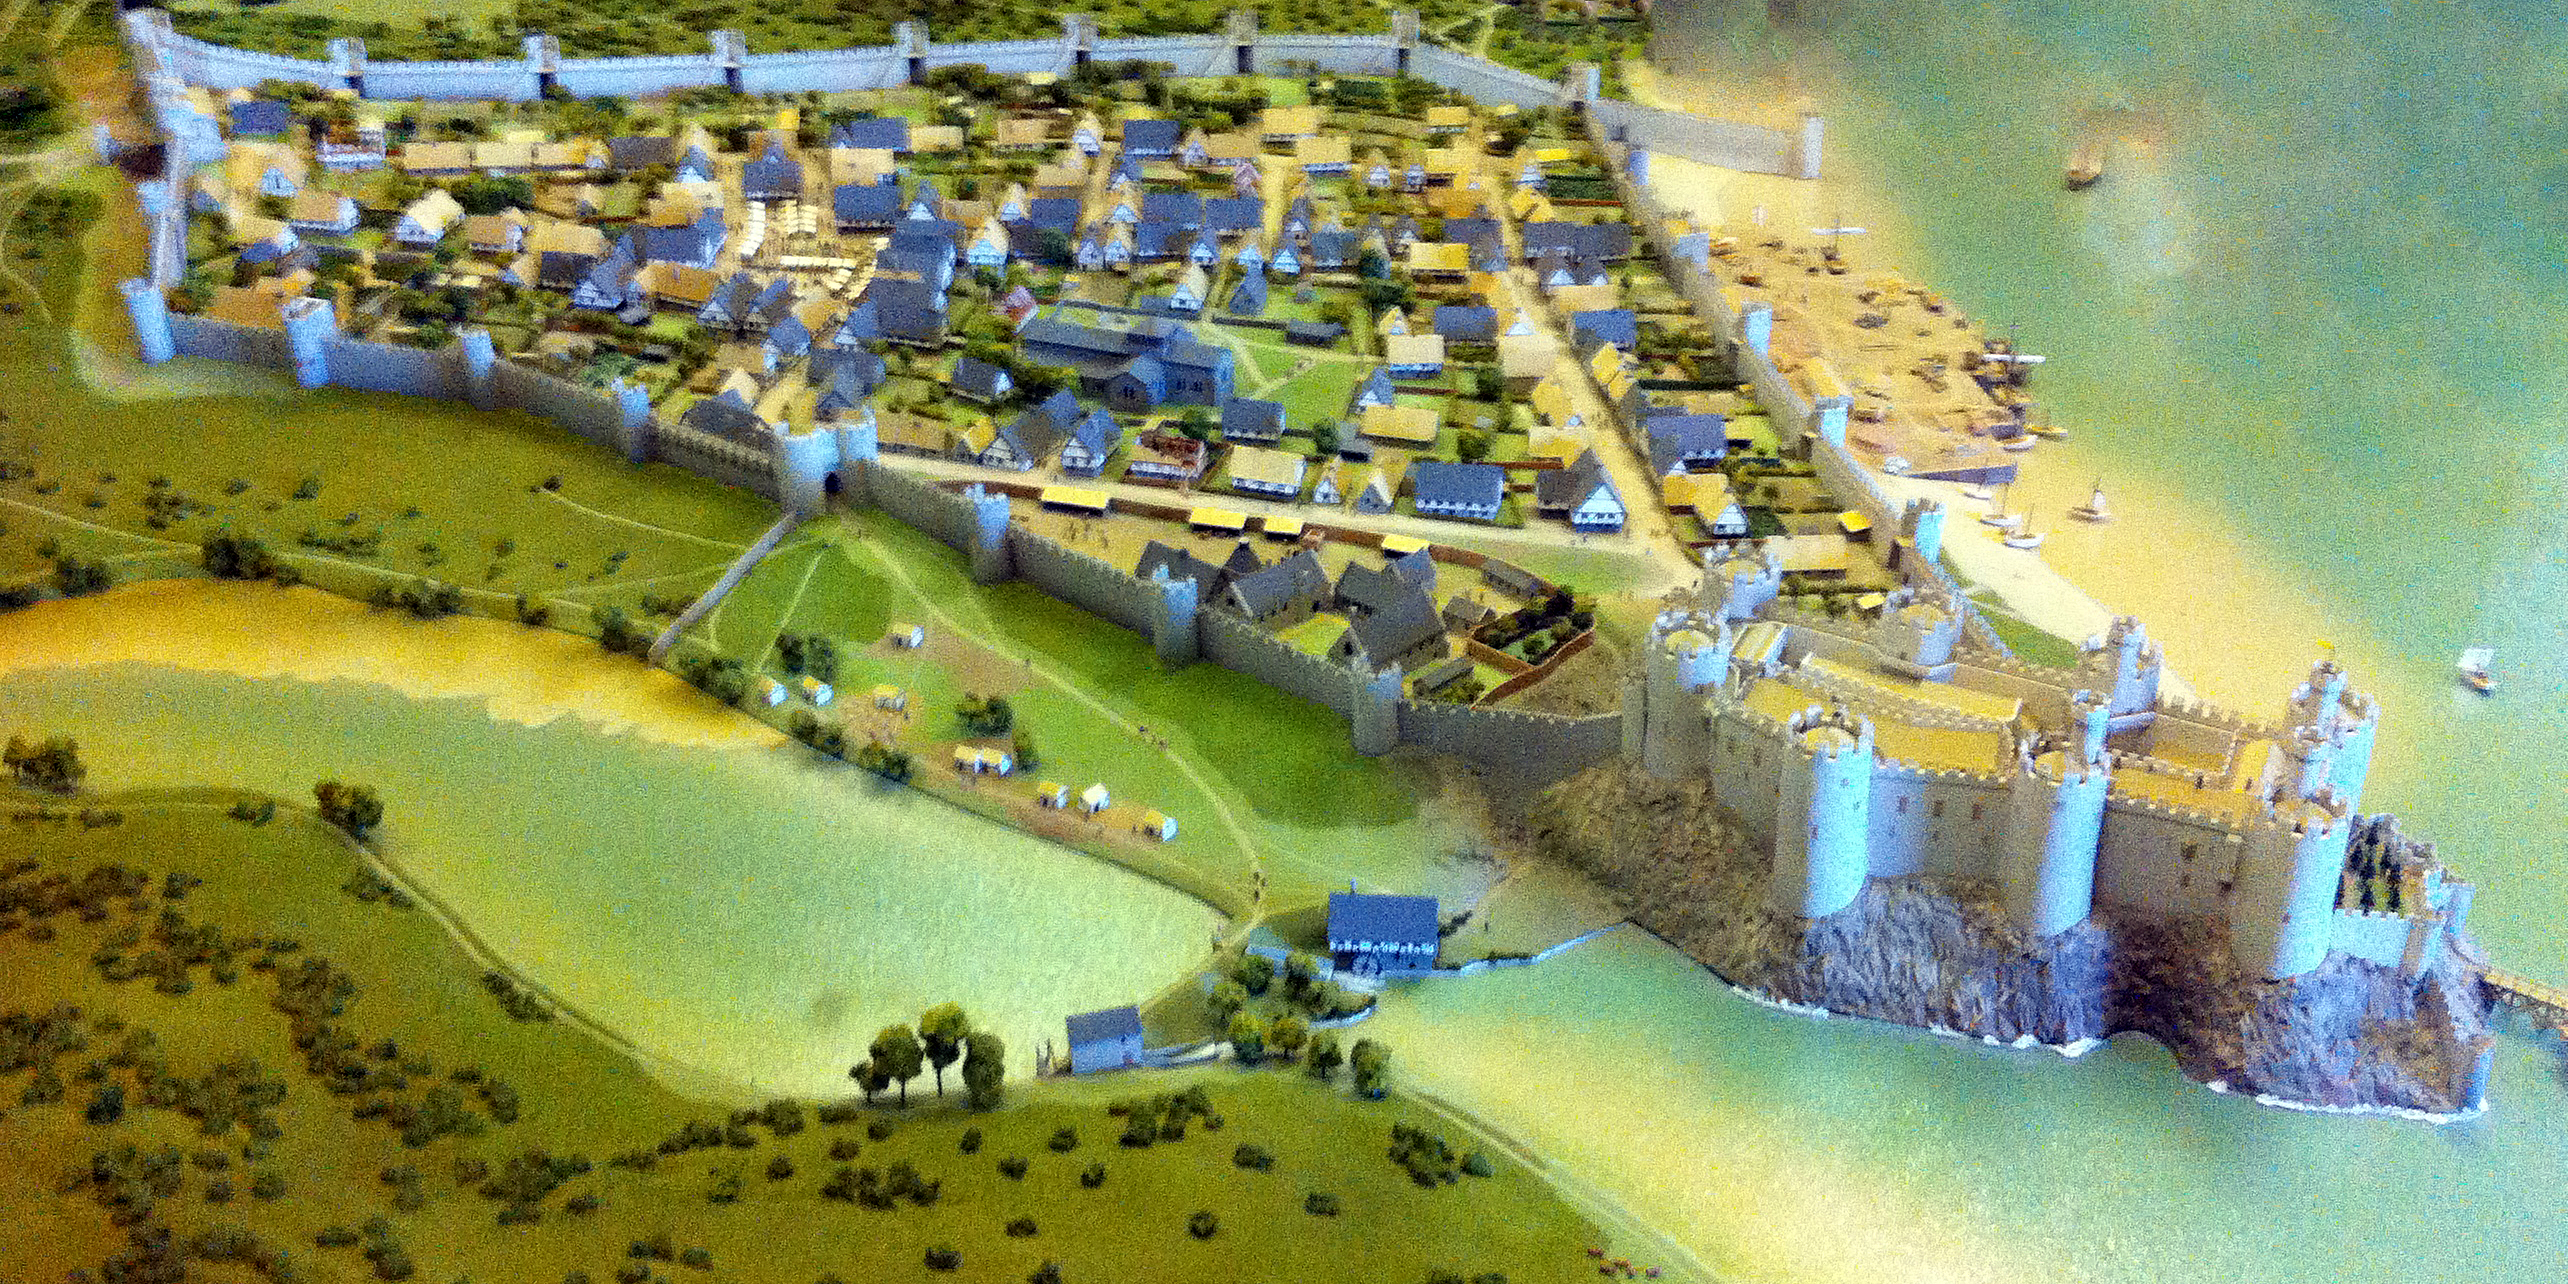
\includegraphics[scale=0.15]{conwycastle1300s.jpg}}
\end{document}

